\section{Near-core structure of a propagating optical vortex \cite{Near16}}
\label{sec:angular_spectrum}
The angular spectrum method is proposed to study the near-core structure of a charge-$1$ optical vortex. Usually, a vortex beam is modeled by Fresnel diffraction  with paraxial approximation, which neglects the effects caused by the radial component of the wavenumber vector. However, a optical vortex presents a significant phase dip in the vicinity of its core, which is mispredicted by the traditional model. The proposed method intrinsictly take not only the propagating but {\em evanescent} frequencies into accounts, where the latter is the main cause for the extra phase dip and is attributed to the neglected radial component of wavenumber vector. In view of this, angular spectrum method provides a clearer picture of the near-core structure and a exact way to simulate it analytically.

\subsection{Backgrounds}
Ever since sigularities of waves have been studied \cite{Ber73}, the skew-dislocations type of singularities have received a lot of attention. 
Typically, a light wave can be modeled as a complex-valued smooth functions $\psi = A e^{i \Phi}$. 
A skew-dislocation or optical vortex occurs when contour lines representing ${\rm Re} \{ \psi \} = 0, {\rm Im} \{ \psi \} = 0$ 
cross each other. 
An important parameter for an optical vortex is the topological charge $m$, defined by (See Appendix I)
\begin{eqnarray}
	&&m = \frac{1}{2\pi} \oint_C \nabla \Phi \cdot d\bar{r} = \frac{1}{2\pi} \oint_C d\Phi
\end{eqnarray}
The phase distribution function for an optical vortex having topological charge $m$ can be represented in the cylindrical coordinates as
(see Appendix I)
\begin{eqnarray}
	&&\Phi(r, \phi, z) = m \phi + \bar{k} \cdot \bar{d},
	\label{eq:phase}
\end{eqnarray}
where $\bar{d} = \hat{r} r + \hat{z} z$ is the position vector. The phase gradient is normally associated with the wavenumber vector $\bar{k}$ as
\begin{eqnarray}
	&&\nabla \Phi = \nabla (\bar{k} \cdot \bar{d}) = \hat{r} k_{r} + \hat{z} k_z = \bar{k}.
\end{eqnarray}

By assuming paraxial approximation, the term $\bar{k} \cdot \bar{d}$ is regarded to be $\bar{k} \cdot \bar{d} = k_z z$; in other words, no $r$-component of the wavenumber vector is present. However, in the study of near-core structure of an optical vortex, a significant phase delay compared to the expected $\Phi = m\phi + k_z z$ is obsersed. The phenomenon is attributed to the prominent radial component of $\bar{k}$ in the vicinity of vortex core \cite{Near16}, about which we will discuss in details in following sections.

\subsection{Angular spectrum method}

To analyze the phase delay, we need to introduce the angular spectrum method. Consider an abitrary complex-valued field $U(x, y, z)$. On a plane $z = z_1$, one can define its counterpart in frequency domain $A(f_x, f_y, z_1)$, which is related to $U(x, y, z_1)$ by the 2D Fourier transformation pair,
\begin{eqnarray}
	A(f_x, f_y, z_1) = \int_{-\infty}^{\infty} \int_{-\infty}^{\infty} U(x, y, z_1)
	e^{-i 2 \pi (f_x x + f_y y)} dx dy
	\nonumber\\
	U(x, y, z_1) = \int_{-\infty}^{\infty} \int_{-\infty}^{\infty} A(f_x, f_y, z_1)
	e^{i 2 \pi (f_x x + f_y y)} df_x df_y.
	\nonumber
\end{eqnarray}
Here the Fourier basis function $e^{i2\pi (f_x x + f_y y)}$ can be interpreted as a plane wave of unit amplitude transmitting with the direction cosines $\cos\theta_x = \lambda f_x$, $\cos\theta_y = \lambda f_y$ and $\cos\theta_z = (1 - (\lambda f_x)^2 - (\lambda f_y)^2)^{1/2}$ \cite{Fo04}. (See Fig. \ref{fig:dirc_cos} for reference on direction cosine.)
% Unable to show figure?
%\begin{figure}[h]
%	\vskip 3 cm
%	\hskip 0.3 cm
%	\special{wmf: direction_cosines.jpg x=4 cm y=3 cm}
%	\caption{Illustration of direction consines.}
%	\label{fig:dirc_cos}
%\end{figure}
\begin{figure}
	\centering
	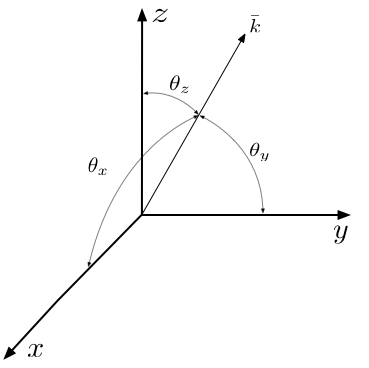
\includegraphics[width = 0.3\textwidth]{direction_cosines.jpg}
	\caption{Illustration of direction consines.}
	\label{fig:dirc_cos}
\end{figure}
With this perspective, the 2-D Fourier transform becomes the decompostion of a field into plane waves with different direction cosines, whence the representation method is called {\em angular spectrum}.


\subsection{Analysis on the propagation of vortex beam}
If the field $U(x, y, z)$ represents an electromagnetc wave, e.g. a vortex beam, then it must satisfy Helmholtz's equation $(\nabla^2 + k^2) U  = 0$. Supposing that $A(f_x, f_y, z)$ is a smooth function in $z$, one can substitute $U$ by the inverse 2-D Fourier transformation of $A$ into Helmholtz's equation and exchange the order of differentiation and integration. Finally, we will end up with the differential equation
\begin{eqnarray}
	\frac{\partial^2 A}{\partial z^2} + \left[ k^2 - 4\pi^2\left( f_x^2 + f_y^2 \right) \right] A= 0,
	\nonumber
\end{eqnarray}
which is in the harmonic form and has the general solution
\begin{eqnarray}
	A(x, y, z) = C(x, y) e^{i (\mu z + \theta)},
	\nonumber
\end{eqnarray}
where $\mu = \sqrt{k^2 - 4\pi^2\left( f_x^2 + f_y^2 \right)}$, $C$ is independent of $z$ and $\theta$ is some constant. Given the initial condition $A(x, y, 0)$, the expression is further reduced to
\begin{eqnarray}
	A(x, y, z) = A(x, y, 0) e^{i \mu z}.
	\label{eq:spectrum_phase}
\end{eqnarray}
If $k^2 \ge 4\pi^2 (f_x^2 + f_y^2)$, $\mu$ will be a real number and Eq. (\ref{eq:spectrum_phase}) then corresponds to a propagating frequency $(f_x, f_y)$. On the other hand, if $k^2 < 4\pi^2 (f_x^2 + f_y^2)$, $\mu$ becomes pure imaginary and Eq. (\ref{eq:spectrum_phase}) will decay as $z$ increases. The latter situation is said to be {\em evanescent}.

By means of Eq. (\ref{eq:spectrum_phase}), the spectrum in two arbitrary transverse planes $z = z_1, z_2$ can be related by $A(f_x, f_y, z_2) = e^{i \mu (z_2 - z_1)} A(f_x, f_y, z_1)$. Having established the angular spectrum method, we can, given the initial field distribution $U(x, y, 0)$, analyze the evolution of vortex beam field $U(x, y, z)$ as $z$ increases by working on the frequency domain,

%\begin{figure}[h]
%	\vskip 3 cm
%	\hskip 0.3 cm
%	\special{wmf: cd.jpg x=4 cm y=3 cm}
%	\caption{The commutation diagram.}
%	\label{fig:commu_diag}
%\end{figure}
\begin{figure}
	\centering
	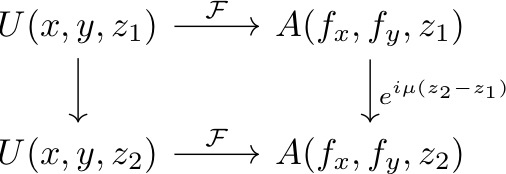
\includegraphics[width = 0.3\textwidth]{cd.jpg}
	\caption{The commutation diagram.}
\end{figure}

Due to the fact that the above commutation diagram commutes, we can obtain the field expression $U(x, y, z)$ given $U(x, y, 0)$ by transforming $U(x, y, 0)$ to frequency-doamin, performing a frequency response of $e^{i \mu z}$ and trasforming the result back to the time-domain. Recall that the field expression of a on-axis vortex beam with $m = 1$ is represented by $\psi = Ce^{i (\phi + k_z z)}$ for some constant $C$. Hence, we may suppose without loss of generousity that $C = 1$ and put $U(x, y, 0) = e^{i\phi}$. The corresponding $A(f_x, f_y, 0)$ can be then computed by 2-D Fourier transformation in cylindrical coordinates (see Appendix II),
\begin{eqnarray}
	A(\rho, \chi, 0) = \frac{-i e^{i\chi}}{2\pi \rho^2},
\end{eqnarray}
where $\rho^2 = f_x^2 + f_y^2$, $ \chi = \arctan(f_y/f_x)$. After a propagation over a distance $z$, the angular spectrum becomes
\begin{eqnarray}
	A(\rho, \chi, z) = \frac{-i e^{i(\mu z + \chi)}}{2\pi \rho^2}.
\end{eqnarray}
Finally, one can obtain the time-domain field by computing the inverse transformation
\begin{eqnarray}
	U(r, \phi, z) =  \int_{0}^{2\pi} \int_{0}^{\infty} \frac{-i e^{i(\mu z + \chi)}}{2\pi \rho^2}e^{i 2\pi \rho r \cos(\chi - \phi)} \rho d\rho d\chi.
	\nonumber
\end{eqnarray}
Note that we have the Jacobi-Anger identity,
\begin{eqnarray}
	e^{ix\cos\theta} = \sum_{n = -\infty}^{\infty} i^n J_{n}(x) e^{i n \theta},
\end{eqnarray}
for arbitrary $x$ and  $\theta \in {\cal R}$. Therefore, we expand the term
\begin{eqnarray}
	e^{i 2 \pi r \rho \cos(\chi - \phi)} = 
	\sum_{n = -\infty}^{\infty} i^{n} J_n(2 \pi r \rho) e^{i n (\chi - \phi)},
	\nonumber
\end{eqnarray}
and notice that $ \int_{0}^{2\pi} e^{i \chi} e^{i n \chi} d\chi = 0$ unless $n = -1$. Hence,
\begin{eqnarray}
	&&U(r, \phi, z) = \int_{0}^{\infty} \frac{- e^{i \mu z}}{2 \pi \rho} \int_{0}^{2\pi} e^{i\phi} J_{-1}(2 \pi r \rho) d\chi d\rho
	\nonumber\\
	&& \hspace{0.5in} = e^{i \phi} \int_{0}^{\infty} \rho^{-1} e^{i \mu z} J_1(2 \pi r \rho) d\rho,
\end{eqnarray}
since $J_{-n} = (-1)^n J_{n}$. Let $I(r, z)$ denote the integral $\int_{0}^{\infty} \rho^{-1} e^{i \mu z} J_1 (2 \pi r \rho) d\rho$, and we get the final result
\begin{eqnarray}
	U(r, \phi, z) = e^{i\phi} I(r, z).
	\label{eq:prop_vortex_beam}
\end{eqnarray}
From Eq. (\ref{eq:prop_vortex_beam}) we can observe the phase part of $I(r, z)$ provides addition phase delay to the original $e^{i \phi}$ term. Moreover, $I(r, z)$ depends on both $r$ and $z$, which is in agreement with the claim that the radial component of wavenumber vector $\bar{k}$ attributes the phase change near vortex core. Subsequently, one can study the behavior of the field near a vortex core by numerically analysing the integral $I(r, z)$.
\subsection{Simulation of phase delay}